% =====================================================================
%  People of the Holocaust -- Database Guide (running document)
%
%  PUBLIC version. Server names, logins and passwords are NOT in this
%  file; they are in the private "Database Handoff Details" document.
%  Placeholders used below: <user>, <server>, <db-user>.
%
%  Formatted to match the Fall 2026 Tool Choices document.
%  Compiles with pdflatex (Overleaf works). Run it twice so the table of
%  contents fills in. figures/schema.png must sit next to this file.
%
%  To update: change the text, add a row to Revision History, bump the
%  version on the title page, recompile.
% =====================================================================

\documentclass[11pt]{article}

\usepackage[letterpaper,margin=1.25in]{geometry}
\usepackage[T1]{fontenc}
\usepackage{lmodern}
\usepackage{array}
\usepackage{longtable}
\usepackage{graphicx}
\usepackage{xcolor}
\usepackage{listings}
\usepackage[hidelinks]{hyperref}

\renewcommand{\arraystretch}{1.25}
\setlength{\parskip}{0.6em}
\setlength{\parindent}{0pt}

% let lines with long code words stretch instead of running into the margin
\sloppy

% column type for wrapping table cells
\newcolumntype{L}[1]{>{\raggedright\arraybackslash}p{#1}}

% inline code
\newcommand{\code}[1]{\texttt{#1}}

% code blocks; literate lets the German names in comments through pdflatex
\lstset{
  basicstyle=\ttfamily\small,
  columns=fullflexible,
  keepspaces=true,
  breaklines=true,
  frame=single,
  rulecolor=\color{gray},
  xleftmargin=0.5em,
  xrightmargin=0.5em,
  literate={ö}{{\"o}}1 {ü}{{\"u}}1 {ä}{{\"a}}1 {Ö}{{\"O}}1 {é}{{\'e}}1
}

% callout box for things that are planned but not built yet
\newcommand{\planned}[1]{%
  \begin{center}\fbox{\parbox{0.92\linewidth}{\textbf{Status:} #1}}\end{center}}

\begin{document}

% =====================================================================
%  TITLE PAGE
% =====================================================================
\begin{titlepage}
\begin{center}

\vspace*{1.2in}

{\LARGE\bfseries People of the Holocaust}\\[0.9em]
{\Large\bfseries Database Guide}\\[0.6em]
{\large Running Document}

\vfill

COSC 4920 - Principles of Design\\[0.6em]
Marquette University\\[1.2em]
Version 0.3\\[0.6em]
\today

\vspace*{0.8in}

\end{center}
\end{titlepage}

% =====================================================================
%  CONTENTS
% =====================================================================
\tableofcontents
\newpage

% =====================================================================
\section{Revision History}

\begin{tabular}{|L{0.8in}|L{1.2in}|L{3.4in}|}
\hline
\textbf{Version} & \textbf{Date} & \textbf{Description} \\
\hline
0.1 & November 13, 2026 & Initial guide: access, schema, loading test data,
querying, planned backend connection. \\
\hline
0.2 & November 13, 2026 & Known Data Issues: articles skipped by the
scraper's title matching, counted for all four volumes; people search
comes from the name index. \\
\hline
0.3 & November 13, 2026 & Moved the skipped-articles analysis to the
separate NLP Known Issues list. \\
\hline
\end{tabular}

% =====================================================================
\section{Introduction}

\subsection{Purpose}

This document explains how to use the \textit{People of the Holocaust}
database: how to reach it, how the tables are laid out, how to load data,
how to look at it, and how we plan to connect it to the interpreter (the
scraper and NLP).

\subsection{A Running Document}

This guide is updated as the project changes. Sections that describe plans
rather than finished work are marked with a \textbf{Status} box. Every
update gets a row in the Revision History.

\subsection{What Is Not in This Document}

The server name, account setup, database user and password are kept in a
separate private document, \textit{Database Handoff Details}, which is not
stored in any repository. Ask a team member for it. In this guide those
values appear as placeholders:

\begin{tabular}{|L{1.2in}|L{4.2in}|}
\hline
\textbf{Placeholder} & \textbf{Meaning} \\
\hline
\code{<user>} & Your own account on the server \\
\hline
\code{<server>} & The server's host name \\
\hline
\code{<db-user>} & The shared database user \\
\hline
\end{tabular}

% =====================================================================
\section{Why MariaDB}

The full evaluation is in the Fall 2026 \textit{Technology Evaluation}
(Tool Choices) document. In short:

\begin{tabular}{|L{1.5in}|L{3.9in}|}
\hline
\textbf{Reason} & \textbf{Detail} \\
\hline
Supabase did not fit &
The previous team used Supabase. Its free tier pauses after seven days of
inactivity, and our site has to show correct information at all times.
We also expect more traffic than the free tier is built for, and we do not
need Supabase's main strength, user authentication, because every visitor
sees the same public information. \\
\hline
Free and open source &
MariaDB needs no license and has no usage cost, so cost does not grow as
the site gets more traffic. \\
\hline
Data stays local &
The data lives on a Marquette Computer Science server. Nothing passes
through a third-party service. \\
\hline
Standard SQL &
Tables, relationships and queries use ordinary SQL, which makes the
project easier to maintain and to pass on. \\
\hline
Easier handoff &
A future team is simply given access to the server, instead of having a
hosted Supabase project transferred to them. \\
\hline
\end{tabular}

% =====================================================================
\section{Accessing the Database}

\subsection{Two Different Logins}

Getting into the database takes two logins, and they use different
passwords:

\begin{enumerate}
  \item \textbf{The server (SSH).} You log in to the server with your own
  university account, \code{<user>}.
  \item \textbf{The database (MariaDB).} Once you are on the server, you log
  in to MariaDB as the shared database user, \code{<db-user>}.
\end{enumerate}

The database password only works for step 2. Typing it at the SSH password
prompt does not work, because the database user is not a server account.
Off campus, connect to the university VPN first.

\subsection{Logging In}

From PowerShell or Windows Terminal (SSH is built into Windows):

\begin{lstlisting}
ssh <user>@<server>
\end{lstlisting}

The first time, type \code{yes} to trust the server. Nothing appears on
screen while you type the password; that is normal. Then log in to the
database:

\begin{lstlisting}
mariadb -u <db-user> -p
\end{lstlisting}

Notes:
\begin{itemize}
  \item \code{mysql} is the old name of the same program. It still works
  but prints a deprecation warning, so use \code{mariadb}.
  \item Running \code{mariadb} \textbf{without} \code{-u} logs you in as an
  anonymous account that cannot see the project database.
  \item If the database user is refused even with the right password, try
  adding \code{-h 127.0.0.1} to the command.
  \item An idle SSH session eventually drops with
  \textit{client\_loop: send disconnect}. Just log in again.
\end{itemize}

\subsection{First Commands}

\begin{lstlisting}
SHOW DATABASES;      -- PotH should be listed
USE PotH;            -- switch into it
SHOW TABLES;
DESCRIBE Paragraph;  -- a table's columns
exit
\end{lstlisting}

Every statement ends with a semicolon; if the prompt changes to \code{->},
MariaDB is waiting for one. Table names are case-sensitive on the server:
\code{Volume} and \code{volume} are different tables.

% =====================================================================
\section{Database Schema}

\subsection{Diagram}

\begin{center}
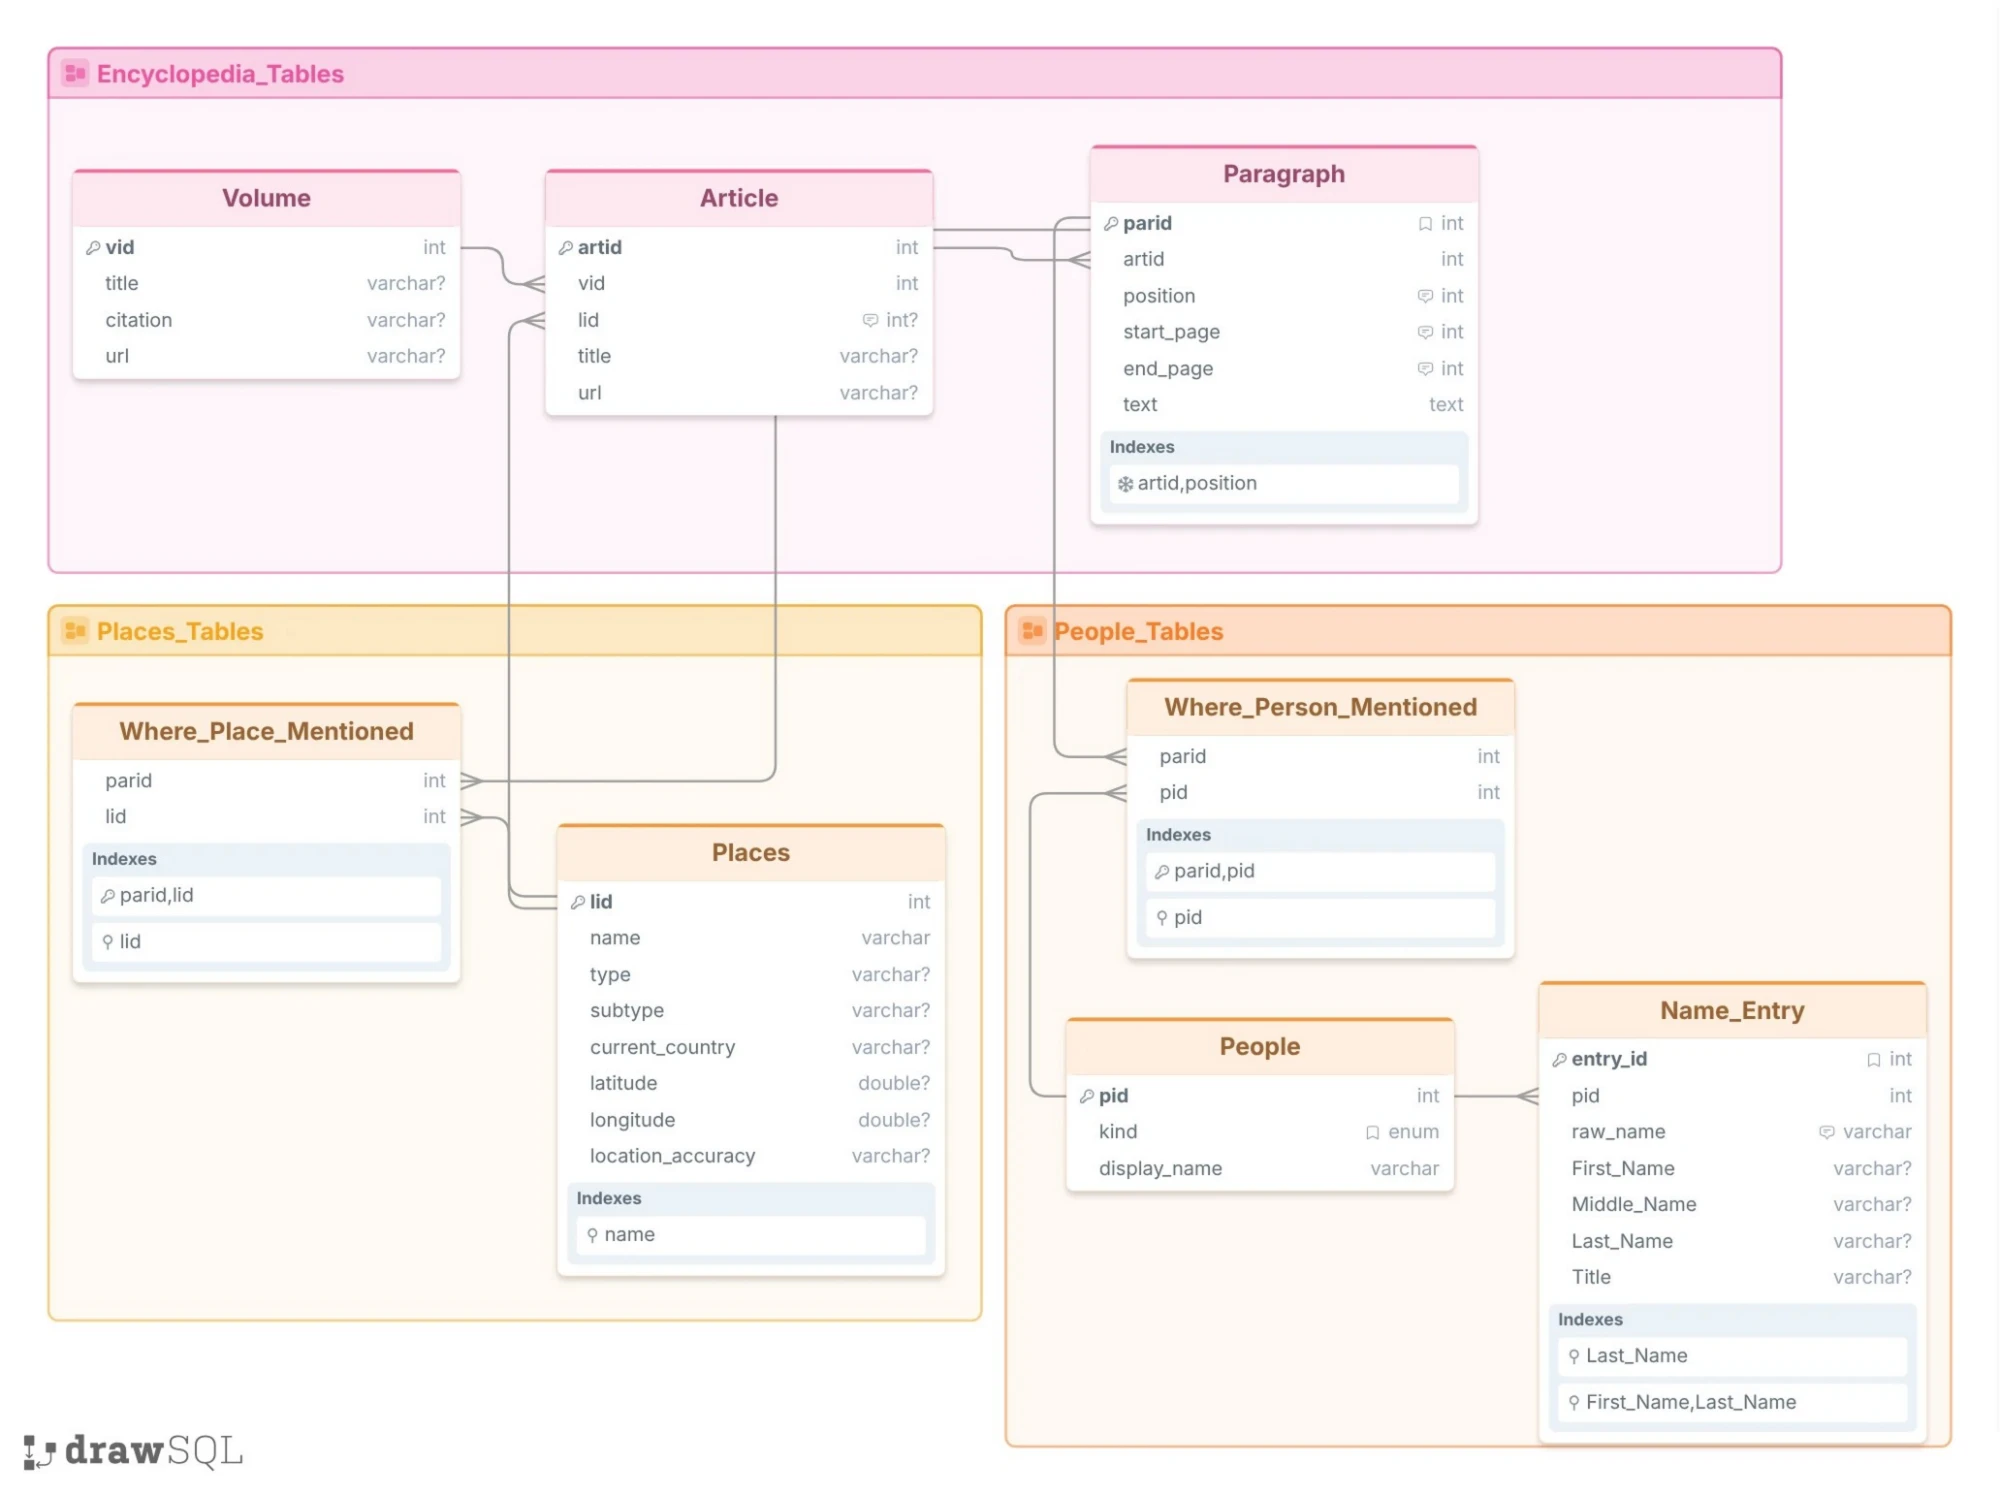
\includegraphics[width=\linewidth]{figures/schema.png}
\end{center}

The tables fall into three groups. The encyclopedia tables hold the text.
The people and places tables hold who and where. The two
\code{Where\_*\_Mentioned} tables link people and places to the
paragraphs they appear in.

\subsection{Tables}

\begin{longtable}{|L{1.95in}|L{3.45in}|}
\hline
\textbf{Table} & \textbf{What one row is} \\
\hline
\endhead
\code{Volume} & One volume of the encyclopedia (\code{vid} 1--4), with its
title, citation and Project MUSE URL. \\
\hline
\code{Article} & One encyclopedia article. \code{artid} is the Project MUSE
document number (\code{/document/1261} becomes 1261). \code{lid} is the place
the article is about, and can be empty. \\
\hline
\code{Paragraph} & One paragraph of an article. \code{parid} is assigned by
the database. \code{(artid, position)} is unique and gives the order within
the article. \code{start\_page} and \code{end\_page} come from the
\code{[End Page N]} markers, so each paragraph can be cited by page. \\
\hline
\code{People} & One person (or family). \code{pid} matches the row index of
\code{people\_table.csv}. \code{kind} is \code{individual}, \code{family} or
\code{brothers}. \\
\hline
\code{Name\_Entry} & One way a person is listed in the encyclopedia's name
index. A person with two spellings gets two rows with the same \code{pid}. \\
\hline
\code{Places} & One place, with type, country and coordinates. \code{lid}
matches the \code{LID} column of \code{place\_table.csv}. \\
\hline
\code{Where\_Person\_Mentioned} & Person \code{pid} is mentioned in
paragraph \code{parid}. The pair is the primary key, so a person is listed
once per paragraph. \\
\hline
\code{Where\_Place\_Mentioned} & Place \code{lid} is mentioned in
paragraph \code{parid}. \\
\hline
\end{longtable}

\subsection{Design Decisions}

\begin{itemize}
  \item \textbf{Mentions are per paragraph.} ``Mentioned together'' means
  appearing in the same paragraph. This matches the Tool Choices document:
  people in close proximity in the text are treated as related.
  \item \textbf{No ``mentioned with'' column.} Who is mentioned with whom,
  and which places are connected to a person, are worked out with queries
  (joins on \code{parid}) rather than stored. Storing them would duplicate
  data and could drift out of sync.
  \item \textbf{Character set \code{utf8mb4}} with collation
  \code{utf8mb4\_unicode\_ci}, so German and Polish names are stored
  correctly. Searches ignore accents: \code{Bohmcker} finds
  \textit{Böhmcker}.
  \item \textbf{Delete rules.} Deleting an article deletes its paragraphs
  and their mentions. Deleting a person deletes their name entries and
  mentions. Deleting a place clears \code{Article.lid} instead of deleting
  the article. A volume that still has articles cannot be deleted.
  \item \textbf{No Activity table.} The previous team's Supabase database
  stored subject--verb--object ``activities''. They are not in this schema.
  Whether to bring them back is still open.
\end{itemize}

The full \code{CREATE TABLE} script is in Appendix~\ref{app:schema}.

% =====================================================================
\section{Repository Files}

The SQL files live in the \code{database/} folder of the
\code{interpreter} repository, on the \code{database-testing} branch.

\begin{tabular}{|L{1.75in}|L{3.65in}|}
\hline
\textbf{File} & \textbf{Purpose} \\
\hline
\code{PoTH.sql} & Drops and recreates all tables, empty. \\
\hline
\code{test\_data.sql} & Practice data as \code{INSERT} statements. \\
\hline
\code{test\_data/} & The same practice data as CSV files (the hand-off
format, Section~\ref{sec:backend}). \\
\hline
\code{load\_test\_data.sql} & Loads the CSV files from \code{test\_data/}
and checks the result. \\
\hline
\code{practice\_queries.sql} & Twelve practice questions with answers. \\
\hline
\code{page\_queries.sql} & The queries behind a search page, a person
page and a place page. \\
\hline
\end{tabular}

The practice data comes from two Volume I articles, Ahrensbök-Holstendorf
(document 1261) and Moringen-Solling, men (document 1330), using the real
\code{pid} and \code{lid} values from the interpreter's CSV tables. The
paragraph text is a short paraphrase, not the encyclopedia's wording.

% =====================================================================
\section{Updating the Database}

\subsection{Copying Files to the Server and Loading Them}

From the \code{interpreter} folder on your own computer:

\begin{lstlisting}
cd <path-to>\interpreter
scp -r database <user>@<server>:~
\end{lstlisting}

This copies the folder to \code{\textasciitilde/database} in your home
folder on the server, replacing older copies of the same files. Then:

\begin{lstlisting}
ssh <user>@<server>
cd ~/database
mariadb --local-infile=1 -u <db-user> -p
\end{lstlisting}

At the MariaDB prompt:

\begin{lstlisting}
source PoTH.sql;
source load_test_data.sql;
\end{lstlisting}

\code{PoTH.sql} rebuilds the empty tables and \code{load\_test\_data.sql}
fills them. The load ends with two checks: an \textit{unmatched mentions}
query that should return \textit{Empty set}, and row counts that should
read 1, 5, 21, 22, 2, 20, 41, 18 for the practice data. The load clears
the tables first, so it can be run as often as needed.

\subsection{Why the Folder and the Flag Matter}

\begin{itemize}
  \item \code{LOAD DATA LOCAL INFILE} finds files relative to the folder
  you were in when you started \code{mariadb}. Start it from
  \code{\textasciitilde/database}.
  \item \code{--local-infile=1} turns on loading local files. Without it
  MariaDB answers \textit{The used command is not allowed with this
  MariaDB version}.
\end{itemize}

\subsection{Backups}

Run from the server shell, not inside MariaDB:

\begin{lstlisting}
mariadb-dump -u <db-user> -p PotH > backup.sql     # save everything
mariadb -u <db-user> -p PotH < backup.sql          # restore it
\end{lstlisting}

% =====================================================================
\section{Looking at the Data}

After logging in to MariaDB:

\begin{itemize}
  \item \code{source practice\_queries.sql;} runs the practice questions,
  from single-table lookups up to joins and ``mentioned with''.
  \item \code{source page\_queries.sql;} shows everything a website page
  would display. Change the \code{SET @pid}, \code{SET @lid} or
  \code{SET @q} line at the top of a section to look at a different person,
  place or search.
  \item End a query with \code{\textbackslash G} instead of \code{;} to
  show each row as a list of fields. This is the easiest way to read
  paragraph text.
  \item \code{pager less -S} makes wide output scroll sideways;
  \code{nopager} turns it off.
  \item If a search fails with \textit{Illegal mix of collations}, run
  \code{SET NAMES utf8mb4 COLLATE utf8mb4\_unicode\_ci;} first.
\end{itemize}

To save a full page's output to a file and read it afterwards (from the
server shell):

\begin{lstlisting}
mariadb -t -u <db-user> -p < page_queries.sql > page_output.txt
less page_output.txt
\end{lstlisting}

For a graphical view, DBeaver (free) can connect with its \textit{SSH
tunnel} option: SSH host \code{<server>} with your own login, database
user \code{<db-user>}. It can browse tables, run queries and draw a
diagram of the live tables. The tunnel avoids opening any ports on the
server.

% =====================================================================
\section{Connecting the Database to the Backend}
\label{sec:backend}

\planned{Idea only, not built yet. The NLP is still being modified.
Revisit this section and update it once the connection is official
(target: mid-December 2026).}

\subsection{Where the Interpreter Runs}

Clone the \code{interpreter} repository onto the server, install it with
\code{pip install .}, and run it there. It then reaches MariaDB on
\code{localhost}, so no ports need to be opened and nothing leaves the
server.

While developing on a laptop instead, an SSH tunnel gives the same access:

\begin{lstlisting}
ssh -L 3307:localhost:3306 <user>@<server>
\end{lstlisting}

Python then connects to \code{127.0.0.1}, port 3307.

\subsection{Hand-off Through CSV Files}

The interpreter writes CSV files shaped like the tables, and
\code{load\_test\_data.sql} (renamed when it is used for real data) loads
them. The interpreter never writes to the database directly.

\begin{longtable}{|L{1.6in}|L{3.8in}|}
\hline
\textbf{File} & \textbf{Columns} \\
\hline
\endhead
\code{articles.csv} & artid, vid, lid, title, url \\
\hline
\code{paragraphs.csv} & artid, position, start\_page, end\_page, text \\
\hline
\code{person\_mentions.csv} & artid, position, pid \\
\hline
\code{place\_mentions.csv} & artid, position, lid \\
\hline
\multicolumn{2}{|l|}{\textit{Reference files, loaded once:}} \\
\hline
\code{volumes.csv} & vid, title, citation, url \\
\hline
\code{places.csv} & lid, name, type, subtype, current\_country, latitude,
longitude, location\_accuracy \\
\hline
\code{people.csv} & pid, kind, display\_name \\
\hline
\code{name\_entries.csv} & pid, raw\_name, First\_Name, Middle\_Name,
Last\_Name, Title \\
\hline
\end{longtable}

File rules: UTF-8 without a byte-order mark, comma separated, a header
row, \code{\textbackslash n} line endings, \code{\textbackslash N} for
empty values (MariaDB reads it as NULL), and no pandas index column.

The interpreter does not know \code{parid}, because the database assigns
it. Mention files therefore name a paragraph by \code{(artid, position)}.
The load script puts them in a temporary staging table and looks up the
real \code{parid} with a join.

\subsection{Why CSV Files and Not Direct Inserts}

Writing straight into the tables would also work, and is not a security
problem when both run on the same server. We chose files because:

\begin{itemize}
  \item \textbf{Easier debugging.} The output can be opened and read before
  it is loaded. Without files we would have to query the database to see
  what the NLP produced.
  \item \textbf{Easier testing.} The loading side can be built and tested
  with hand-made files while the NLP is still changing.
  \item \textbf{Backups.} The files are a copy of each run. If the
  database is damaged, reload them.
  \item \textbf{Separation.} The NLP team only has to produce the agreed
  files. They never touch SQL.
\end{itemize}

\subsection{Changes Needed in the Interpreter}

\begin{itemize}
  \item It currently signs in to Supabase and inserts only activity rows
  into an \code{Activity} table (\code{data\_structure.py}). That code is
  replaced by writing the CSV files.
  \item Keep paragraph breaks. The text is currently split straight into
  sentences.
  \item Keep the \code{[End Page N]} markers long enough to record page
  numbers. \code{clean\_article} currently deletes them.
  \item Record the paragraph each person is found in, not just the
  sentence.
  \item Detect places in the text. Nothing does this yet.
\end{itemize}

\subsection{If a Direct Connection Is Needed Later}

Use the PyMySQL package, keep credentials in \code{.env} (protected with
\code{chmod 600} and listed in \code{.gitignore}), always use
parameterized queries (\code{\%s}) because the text is full of
apostrophes, and commit one article per transaction.

% =====================================================================
\section{Why a Database and Not Just CSV Files}

The CSV files carry data from the interpreter to the database. The
database is where the data lives.

\begin{itemize}
  \item \textbf{It refuses bad data.} A CSV accepts anything. The database
  rejects a mention of a person who does not exist, a duplicate mention, or
  a wrong value type.
  \item \textbf{Joins.} Questions that span several tables, such as every
  place connected to a person with page citations, are a single query.
  \item \textbf{Speed.} Indexes find one person's mentions without reading
  every row, which matters at full encyclopedia size.
  \item \textbf{The website can use it.} A database server handles many
  visitors searching at once.
  \item \textbf{Security.} Backups are simple, and the website can be given
  a login that can only read.
\end{itemize}

% =====================================================================
\section{Known Data Issues}

Problems in the interpreter (the scraper and NLP), including the articles
the scraper never processes, are tracked in a separate \textit{NLP Known
Issues} list. This section covers the data itself.

\begin{itemize}
  \item The people search is built from the encyclopedia's name index
  (\code{people\_table.csv}), not from what the parser finds, so being
  listed there does not mean the parser found the person in an article.
  The name index also links people to articles where they appear only in
  SOURCES or NOTES; for example, it links Hannah Vogt to document 1330,
  where she is only in the sources. Our \code{Where\_Person\_Mentioned}
  table uses article bodies only, so it does not have this problem. The
  scraper already ignores SOURCES and NOTES, which sit outside the article
  body on each page.
  \item The coordinates for Moringen-Solling in \code{place\_table.csv}
  (52.6, 11.75) are wrong; Moringen is near 51.70, 9.87.
  \item Names without a first name, such as Müller, match many people.
  The interpreter cannot decide between them yet.
  \item Some people have two index entries (for example
  \textit{Wolten-Pecksen, Otto} and \textit{Pecksen: Wolten-Pecksen,
  Otto}). They should share one \code{pid}.
  \item Place names are not unique across time: the Osnabrück rows in
  \code{place\_table.csv} are later subcamps, not the 1933 site.
\end{itemize}

% =====================================================================
\section{Open Items}

\begin{itemize}
  \item Update Section~\ref{sec:backend} once the backend connection is
  official (target: mid-December 2026).
  \item Change the article matching in \code{scrape\_articles.py} so
  skipped articles are processed (see the NLP Known Issues list).
  \item Decide whether the Activity data returns as a table.
  \item Load the full \code{people\_table.csv} and \code{place\_table.csv}.
  \item Create a read-only database user for the website.
\end{itemize}

% =====================================================================
\appendix
\section{Schema Script (\code{PoTH.sql})}
\label{app:schema}

\begin{lstlisting}[language=SQL]
USE PotH;

ALTER DATABASE PotH CHARACTER SET utf8mb4 COLLATE utf8mb4_unicode_ci;

-- Drop everything so this file can be re-run from scratch
SET FOREIGN_KEY_CHECKS = 0;
DROP TABLE IF EXISTS Where_Place_Mentioned, Where_Person_Mentioned,
                     Name_Entry, People, Paragraph, Article, Places, Volume;
SET FOREIGN_KEY_CHECKS = 1;

CREATE TABLE Volume (
  vid       INT PRIMARY KEY,
  title     VARCHAR(255),
  citation  VARCHAR(500),
  url       VARCHAR(500)
) ENGINE=InnoDB DEFAULT CHARSET=utf8mb4 COLLATE=utf8mb4_unicode_ci;

CREATE TABLE Places (
  lid                INT PRIMARY KEY,
  name               VARCHAR(255) NOT NULL,
  type               VARCHAR(100),
  subtype            VARCHAR(100),
  current_country    VARCHAR(100),
  latitude           DOUBLE,
  longitude          DOUBLE,
  location_accuracy  VARCHAR(50),
  INDEX idx_places_name (name)
) ENGINE=InnoDB DEFAULT CHARSET=utf8mb4 COLLATE=utf8mb4_unicode_ci;

CREATE TABLE Article (
  artid  INT PRIMARY KEY,
  vid    INT NOT NULL,
  lid    INT,                      -- the place this article is about
  title  VARCHAR(255),
  url    VARCHAR(500),
  FOREIGN KEY (vid) REFERENCES Volume(vid),
  FOREIGN KEY (lid) REFERENCES Places(lid) ON DELETE SET NULL
) ENGINE=InnoDB DEFAULT CHARSET=utf8mb4 COLLATE=utf8mb4_unicode_ci;

CREATE TABLE Paragraph (
  parid       INT AUTO_INCREMENT PRIMARY KEY,
  artid       INT NOT NULL,
  `position`  INT NOT NULL,        -- order within the article
  start_page  INT NOT NULL,        -- from the [End Page N] markers
  end_page    INT NOT NULL,        -- same as start_page unless it crosses a page break
  `text`      TEXT NOT NULL,
  UNIQUE KEY uq_paragraph_artid_position (artid, `position`),
  FOREIGN KEY (artid) REFERENCES Article(artid) ON DELETE CASCADE
) ENGINE=InnoDB DEFAULT CHARSET=utf8mb4 COLLATE=utf8mb4_unicode_ci;

CREATE TABLE People (
  pid           INT PRIMARY KEY,
  kind          ENUM('individual', 'family', 'brothers') NOT NULL DEFAULT 'individual',
  display_name  VARCHAR(255) NOT NULL
) ENGINE=InnoDB DEFAULT CHARSET=utf8mb4 COLLATE=utf8mb4_unicode_ci;

-- Each name a person is listed under is its own row (e.g. Göth and Goeth -> same pid)
CREATE TABLE Name_Entry (
  entry_id     INT AUTO_INCREMENT PRIMARY KEY,
  pid          INT NOT NULL,
  raw_name     VARCHAR(255) NOT NULL,   -- exactly as in the encyclopedia name index
  First_Name   VARCHAR(100),
  Middle_Name  VARCHAR(100),
  Last_Name    VARCHAR(100),
  Title        VARCHAR(100),
  INDEX idx_name_last (Last_Name),
  INDEX idx_name_first_last (First_Name, Last_Name),
  FOREIGN KEY (pid) REFERENCES People(pid) ON DELETE CASCADE
) ENGINE=InnoDB DEFAULT CHARSET=utf8mb4 COLLATE=utf8mb4_unicode_ci;

CREATE TABLE Where_Person_Mentioned (
  parid  INT NOT NULL,
  pid    INT NOT NULL,
  PRIMARY KEY (parid, pid),
  INDEX idx_wpm_pid (pid),
  FOREIGN KEY (parid) REFERENCES Paragraph(parid) ON DELETE CASCADE,
  FOREIGN KEY (pid)   REFERENCES People(pid)      ON DELETE CASCADE
) ENGINE=InnoDB DEFAULT CHARSET=utf8mb4 COLLATE=utf8mb4_unicode_ci;

CREATE TABLE Where_Place_Mentioned (
  parid  INT NOT NULL,
  lid    INT NOT NULL,
  PRIMARY KEY (parid, lid),
  INDEX idx_wplm_lid (lid),
  FOREIGN KEY (parid) REFERENCES Paragraph(parid) ON DELETE CASCADE,
  FOREIGN KEY (lid)   REFERENCES Places(lid)      ON DELETE CASCADE
) ENGINE=InnoDB DEFAULT CHARSET=utf8mb4 COLLATE=utf8mb4_unicode_ci;
\end{lstlisting}

\end{document}
